\subsection{Combinación de reguladores L78XX y L79XX}
Es posible combinar ambos reguladores positivo y negativo para incrementar la
salida de voltaje, como se muestra en la \textbf{figura~\ref{circuito11}}.

\begin{figure}[!h]
\centering
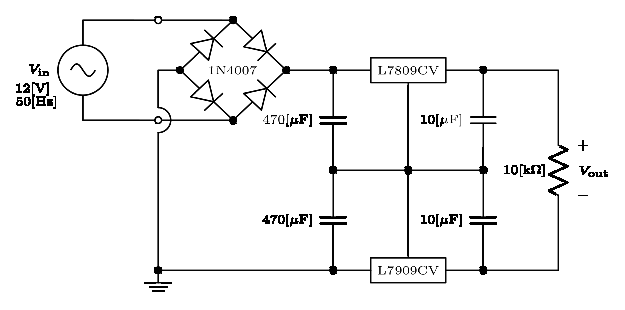
\includegraphics[scale=1.1]{diagramas/11.regulador3.eps}
\caption{Regulación de voltaje con dos circuitos integrados.}
\label{circuito11}
\end{figure}

\subsubsection{Simulación}
Se utilizó el software \emph{Quite Universal Circuit Simulator.} versión 23.3.1
para la simulación de la regulación de voltaje por medio de dos rectificadores,
este puede verse en la \textbf{figura~\ref{simulacion11}}.

\begin{figure}[!h]
\centering
\includegraphics[scale=0.75]{simulacion/11.regulador3.eps}
\caption{Simulación del regulador combinado.}
\label{simulacion11}
\end{figure}

\begin{figure}[!h]
\centering
\includegraphics[scale=0.26]{fotos/11.regulador3.eps}
\caption{Regulador combinado, salida del osciloscopio\\
y medición de voltaje y corriente.}
\label{laboratorio13}
\end{figure}

\subsubsection{Laboratorio}
Se presenta el regulador con dos circuitos integrados armado en laboratorio, su
señal de voltaje de salida en osciloscopio, así como su voltaje y corriente en
un multímetro para una resistencia de carga de $10[\text{k}\Omega]$ en la
\textbf{figura~\ref{laboratorio13}}.

